\documentclass{article}
\usepackage{graphicx}

\begin{document}
\section{Results}
To be sure about the quality of the juxtacellular recording, auto-correlograms were computed for each recording (Fig. \ref{fig:AC}).
\begin{figure}[!h]
	\centering
	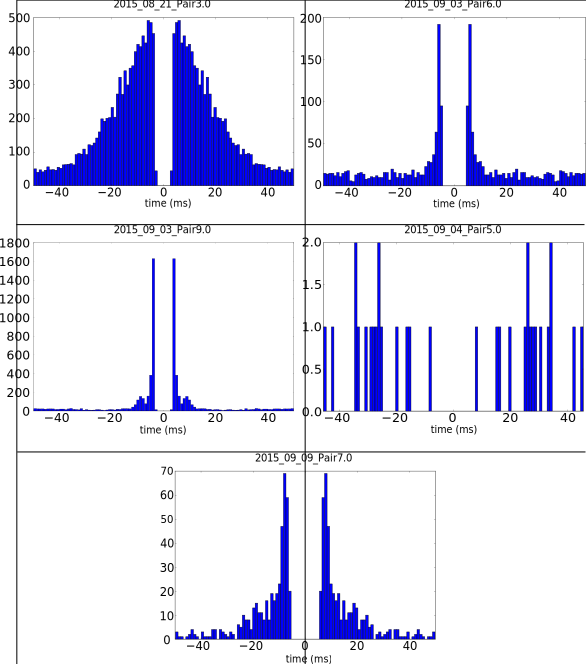
\includegraphics[width=\linewidth]{AC.pdf}
	\caption{Auto-Correlograms for all the recordings. The size of the bins in the histograms is 1 ms and the value for the lag is 50ms.
}
\label{fig:AC}
\end{figure}

All the auto-correlograms display a usual distribution, clearly showing a gap in the interval from -5ms to 5ms, assuring that the cell never spiked twice  within a 5ms interval, which conforms with the typical values of refractory period of 2-3ms.

It is worth noting that on the auto-correlogram corresponding to the recording 939 a second peak is resolved around $\tau = -9 ms$ and $\tau = 9 ms$.

For each recording, phy was run with the following parameters:
The data was filtered with a forwards-backwards Butterworth filter of order 3 with cutoff frequency set to 500Hz. The noise standard deviation was evaluated in 50 excerpts of 1 second each. The weak threshold was $\theta_w = 2 \sigma_{noise}$ and the strong threshold was $\theta_s = 4.5 \sigma_{noise}$.

The results are presented in table REFERENCE.

\begin{table}[!h]

\begin{center}
\begin{tabular}{ccccc}
Recording ID & \# detected Spikes & $\sigma_{noise}$ ($\mu V$) & $\theta_W$ ($\mu V$) & $\theta_S$ ($\mu V$) \\ \hline
8213 & 148762 &  12.95 & 25.91 & 58.30 \\ 
936 & 323629 & 10.76 & 21.52 & 48.43 \\ 
939 & 265476 & 10.51 & 21.02 & 47.29 \\ 
945 & 126234 & 10.92 & 21.84 & 49.14 \\ 
997 & 156932 & 11.47 & 22.93 & 51.60 \\ 
\end{tabular}
\end{center}
\caption{Summary of the output from phy. In this table are the values of the estimated standard deviations of the noise, and the calculated weak and strong thresholds for each recording. These values were converted into $\mu V$.}
\label{tab:results-from-phy}
\end{table}

For each detected spike, all electrodes whose corresponding mask value was non-zero were used.

In Fig. \ref{fig:CC} are the whole-probe cross-correlograms for the recordings.

\begin{figure}[!h]
	\centering
	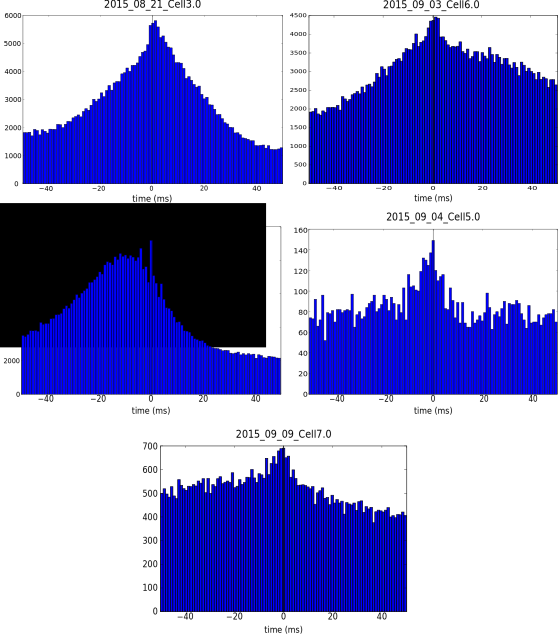
\includegraphics[width=\linewidth]{CC.pdf}
	\caption{Cross-Correlograms for all the recordings. The size of the bins in the histograms is 1 ms and the value for the lag is 50ms.
}
\label{fig:CC}
\end{figure}

In Appendix NUMBEROFAPPENDIX are the cross-correlograms per channel, where the spike train output by phy was splitted according to the electrode the spike was detected on using the masks.

\end{document}